% Penjelasan bertahap metode cosine dosen: cosine, sudut, contoh 2D, kerucut di dimensi tinggi, dan resep.
% Kompilasi (dari folder ini): pdflatex cosine_langkah.tex && pdftoppm -png -r 300 -singlefile cosine_langkah.pdf cosine_langkah
\documentclass[border=6pt]{standalone}
\usepackage{amssymb}
\usepackage{mathptmx}
\usepackage{tikz}
\usetikzlibrary{arrows.meta, calc, positioning}

\definecolor{ink}{HTML}{3A3936}
\definecolor{muted}{HTML}{8A8984}
\definecolor{dataF}{HTML}{F0EFEC}
\definecolor{modelE}{HTML}{2A78D6}\definecolor{modelF}{HTML}{DCE9F9}
\definecolor{augE}{HTML}{EB6834}\definecolor{augF}{HTML}{FDE3D6}

\tikzset{
  every node/.style={font=\small, text=ink, align=center},
  title/.style={font=\small\bfseries, anchor=west},
  vec/.style={-{Stealth[length=2.4mm]}, line width=1.5pt},
  proj/.style={dashed, line width=0.8pt, draw=muted},
  note/.style={font=\footnotesize\itshape, text=muted},
  box/.style={rectangle, rounded corners=3pt, line width=0.8pt, draw=muted, fill=white, inner sep=4pt, text width=76mm, minimum height=11mm},
  flow/.style={-{Stealth[length=2.3mm]}, line width=0.8pt, draw=ink},
}
\newcommand{\sub}{\footnotesize\color{muted}}

\begin{document}
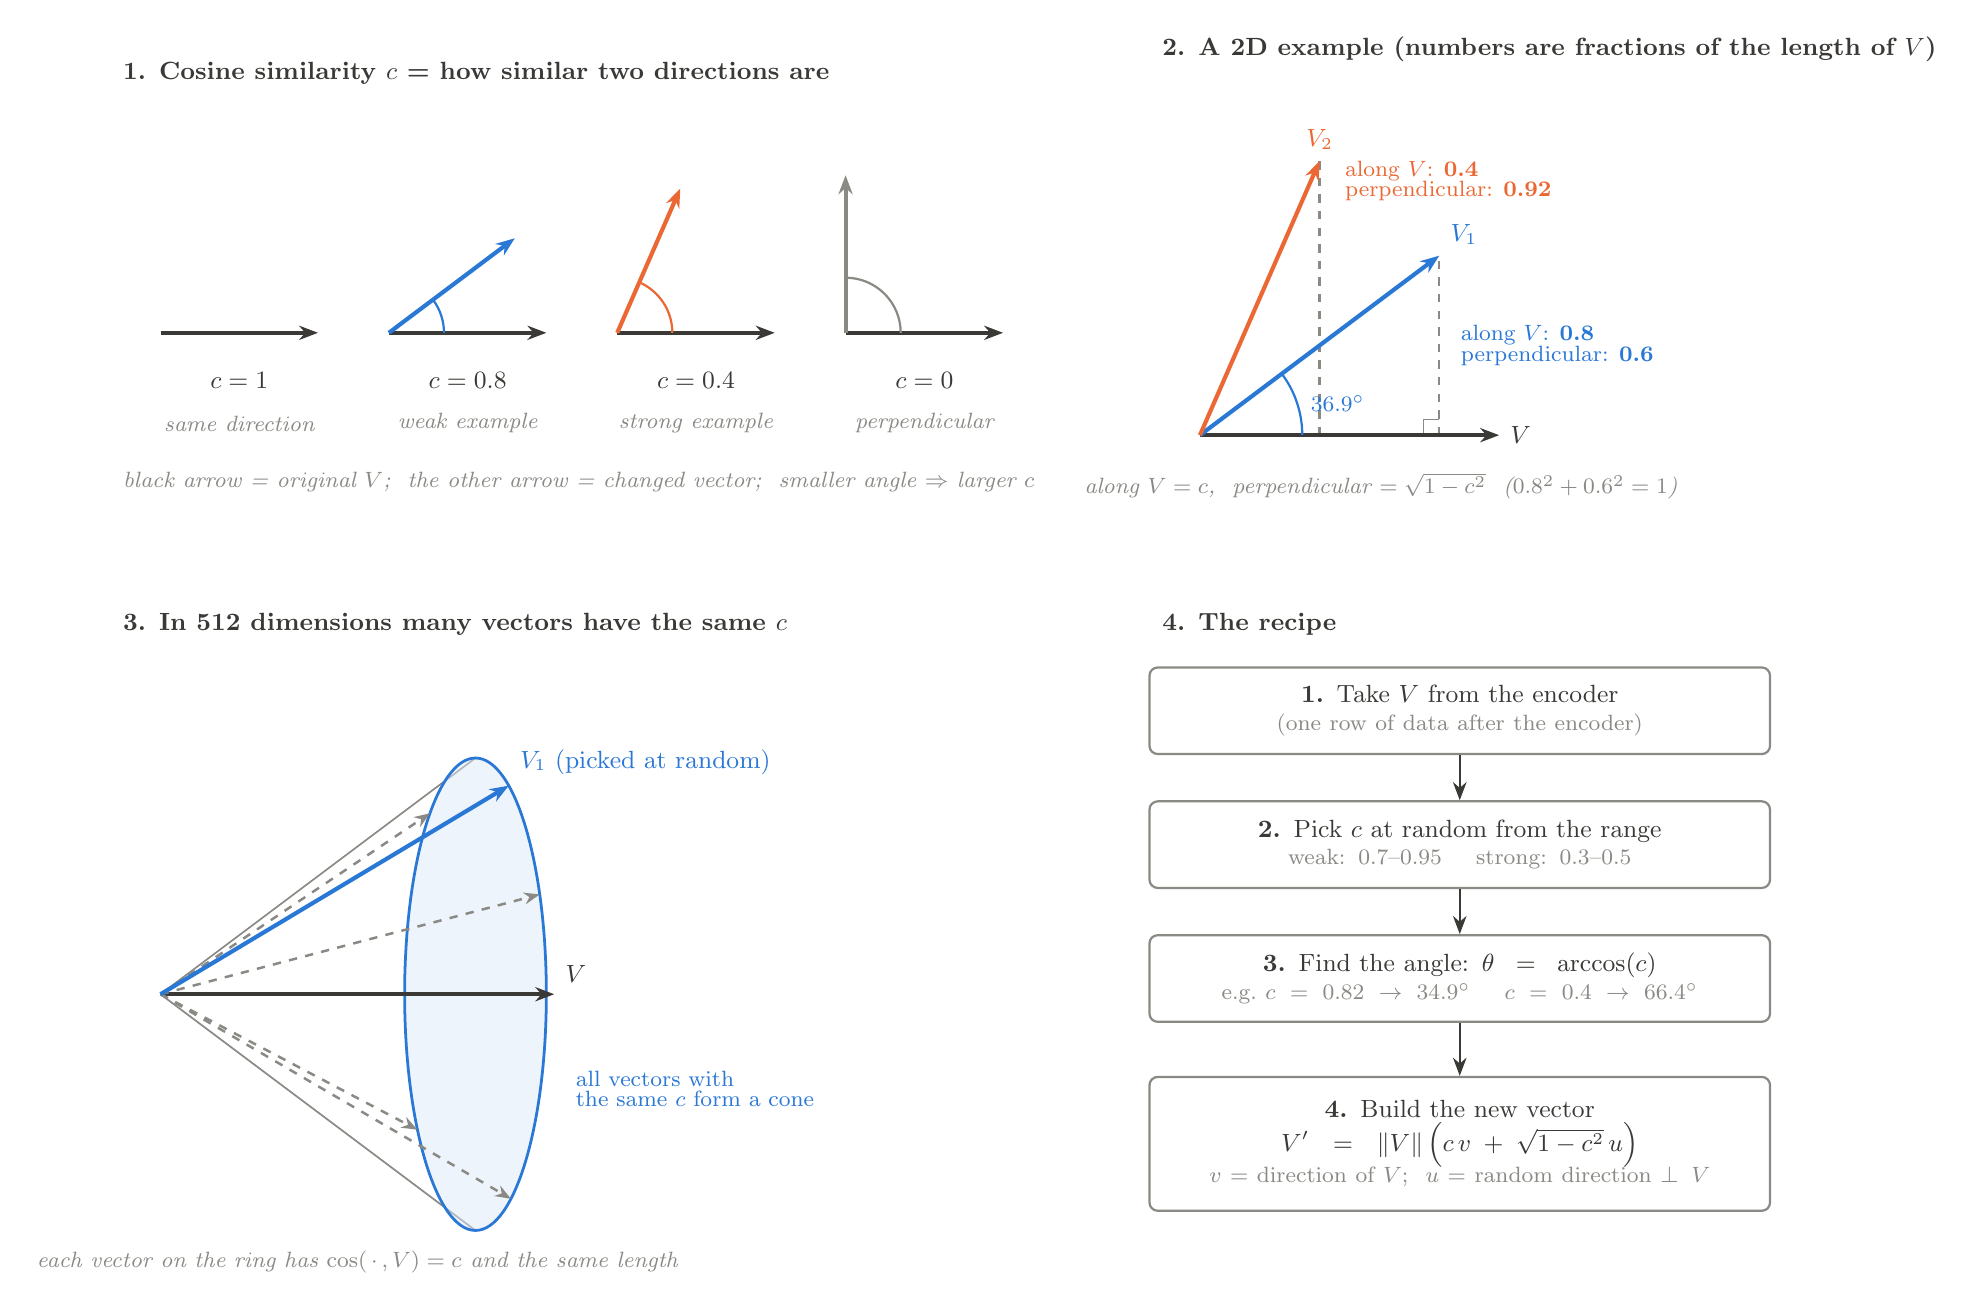
\begin{tikzpicture}

% ============ 1. cosine = kemiripan arah ============
\node[title] at (-0.6, 3.3) {1. Cosine similarity $c$ = how similar two directions are};
\foreach \x/\ang/\col/\lab/\cap in {0/0/muted/{$c=1$}/{same direction}, 2.9/36.9/modelE/{$c=0.8$}/{weak example},
                                    5.8/66.4/augE/{$c=0.4$}/{strong example}, 8.7/90/muted/{$c=0$}/{perpendicular}} {
  \draw[vec, ink] (\x,0) -- (\x+2.0,0);
  \ifdim \ang pt>0pt
    \draw[vec, \col] (\x,0) -- ($(\x,0)+(\ang:2.0)$);
    \draw[\col, line width=0.8pt] ($(\x,0)+(0.7,0)$) arc (0:\ang:0.7);
  \fi
  \node[font=\small] at (\x+1.0,-0.6) {\lab};
  \node[note] at (\x+1.0,-1.15) {\cap};
}
\node[note, anchor=west] at (-0.6,-1.9) {black arrow = original $V$;\ \ the other arrow = changed vector;\ \ smaller angle $\Rightarrow$ larger $c$};

% ============ 2. contoh 2D ============
\begin{scope}[shift={(13.2,-1.3)}]
  \node[title] at (-0.6,4.9) {2. A 2D example (numbers are fractions of the length of $V$)};
  \def\L{3.8}
  % V1: c=0.8 -> (0.8,0.6); V2: c=0.4 -> (0.4,0.9165)
  \draw[proj] (0.8*\L,0) -- (0.8*\L,0.6*\L);
  \draw[proj] (0.4*\L,0) -- (0.4*\L,0.9165*\L);
  \draw[muted, line width=0.6pt] (0.8*\L-0.2,0) -- (0.8*\L-0.2,0.2) -- (0.8*\L,0.2);
  \draw[vec, ink]    (0,0) -- (\L,0) node[right] {$V$};
  \draw[vec, modelE] (0,0) -- (0.8*\L,0.6*\L) node[above right, text=modelE] {$V_1$};
  \draw[vec, augE]   (0,0) -- (0.4*\L,0.9165*\L) node[above, text=augE] {$V_2$};
  \draw[modelE, line width=0.8pt] (1.3,0) arc (0:36.9:1.3);
  \node[font=\footnotesize, text=modelE] at (1.75,0.4) {$36.9^\circ$};
  \node[font=\footnotesize, text=modelE, anchor=west, align=left] at (0.8*\L+0.15,0.3*\L) {along $V$: \textbf{0.8}\\[-2pt]perpendicular: \textbf{0.6}};
  \node[font=\footnotesize, text=augE, anchor=west, align=left] at (0.4*\L+0.2,0.85*\L) {along $V$: \textbf{0.4}\\[-2pt]perpendicular: \textbf{0.92}};
  \node[note] at (2.3,-0.65) {along $V=c$, \ perpendicular $=\sqrt{1-c^2}$ \ ($0.8^2+0.6^2=1$)};
\end{scope}

% ============ 3. dimensi tinggi ============
\begin{scope}[shift={(0,-8.4)}]
  \node[title] at (-0.6,4.7) {3. In 512 dimensions many vectors have the same $c$};
  \def\L{5.0}
  \def\ax{0.8*\L}\def\ay{0.6*\L}
  % kerucut
  \draw[muted, line width=0.6pt] (0,0) -- (\ax,\ay);
  \draw[muted, line width=0.6pt] (0,0) -- (\ax,-\ay);
  \draw[modelE, line width=1pt, fill=modelF, fill opacity=0.5] (\ax,0) ellipse (0.9 and \ay);
  \draw[vec, ink] (0,0) -- (\L,0) node[above right] {$V$};
  % kandidat vektor di cincin
  \foreach \t in {25,130,215,300} {
    \draw[-{Stealth[length=2mm]}, line width=0.9pt, draw=muted, dashed] (0,0) -- ({\ax+0.9*cos(\t)},{\ay*sin(\t)});
  }
  \draw[vec, modelE] (0,0) -- ({\ax+0.9*cos(62)},{\ay*sin(62)}) node[above right, text=modelE] {$V_1$ (picked at random)};
  \node[font=\footnotesize, text=modelE, anchor=west, align=left] at (\ax+1.15,-1.2) {all vectors with\\[-2pt]the same $c$ form a cone};
  \node[note] at (2.5,-3.4) {each vector on the ring has $\cos(\,\cdot\,,V)=c$ and the same length};
\end{scope}

% ============ 4. resep ============
\begin{scope}[shift={(13.2,-8.4)}]
  \node[title] at (-0.6,4.7) {4. The recipe};
  \node[box] (r1) at (3.3,3.6) {\textbf{1.} Take $V$ from the encoder\\[-1pt]{\sub (one row of data after the encoder)}};
  \node[box] (r2) at (3.3,1.9) {\textbf{2.} Pick $c$ at random from the range\\[-1pt]{\sub weak: 0.7--0.95 \ \ \ strong: 0.3--0.5}};
  \node[box] (r3) at (3.3,0.2) {\textbf{3.} Find the angle: $\theta=\arccos(c)$\\[-1pt]{\sub e.g.\ $c=0.82\to34.9^\circ$ \ \ \ $c=0.4\to66.4^\circ$}};
  \node[box, minimum height=17mm] (r4) at (3.3,-1.9) {\textbf{4.} Build the new vector\\[1pt]$V'=\|V\|\,\bigl(c\,v+\sqrt{1-c^2}\,u\bigr)$\\[-1pt]{\sub $v$ = direction of $V$;\ \ $u$ = random direction $\perp V$}};
  \draw[flow] (r1) -- (r2);
  \draw[flow] (r2) -- (r3);
  \draw[flow] (r3) -- (r4);
\end{scope}

\end{tikzpicture}
\end{document}
